\documentclass[11pt]{article}

\usepackage[T1]{fontenc}
\usepackage{geometry}
\usepackage{amsmath, amssymb, amsthm}
\usepackage{listings}
% \usepackage{courier}
\usepackage{xcolor}
\usepackage{graphicx}
\usepackage{fancyhdr}
\usepackage{lipsum}
% \usepackage{subfigure}
\usepackage{caption}
\usepackage{subcaption}
\usepackage{float}
\usepackage{hyperref}

\makeatletter
\renewcommand\@biblabel[1]{}
\renewenvironment{thebibliography}[1]
     {\section*{\refname}%
      \@mkboth{\MakeUppercase\refname}{\MakeUppercase\refname}%
      \list{}%
           {\leftmargin0pt
            \@openbib@code
            \usecounter{enumiv}}%
      \sloppy
      \clubpenalty4000
      \@clubpenalty \clubpenalty
      \widowpenalty4000%
      \sfcode`\.\@m}
     {\def\@noitemerr
       {\@latex@warning{Empty `thebibliography' environment}}%
      \endlist}
\makeatother

% \captionsetup[table]{skip=10pt}

\geometry{a4paper, margin=1in, headheight=14pt}

\pagestyle{fancy}
\renewcommand\headrulewidth{0.4pt}
\fancyhead[L]{\scshape Experiment IV}
% \lhead{Experiment I}
\rhead{}
\cfoot{\thepage}

\definecolor{darkgreen}{rgb}{0.2, 0.6, 0.4}
\definecolor{darkblue}{rgb}{0.2, 0.4, 0.8}
\lstset{ 
  basicstyle=\footnotesize\ttfamily,
  commentstyle=\color{gray},
  % extendedchars=true,
  % keepspaces=true,
  keywordstyle=\color{darkblue},
  % numbers=left,
  % numbersep=5pt,
  % numberstyle=\tiny\color{gray},
  stringstyle=\color{darkgreen},
  tabsize=4,
  % frame=lines,
  aboveskip=2em,
  belowskip=2em,
  breaklines=true
}

\newcommand\pp[2]{\frac{\partial #1}{\partial #2}}
\newcommand\E[1]{\langle #1 \rangle}

\title{
        \Large\textsc{PH2103: Physics Laboratory III} \\
        \vspace{10pt}
        \Huge \textbf{Amplitude modulation and Superposition} \\
        \vspace{5pt}
        \large{Determination of the velocity of light in different media.}
}
\author{
        \large Satvik Saha%
        \thanks{Email: \tt ss19ms154@iiserkol.ac.in}
        \\\textsc{\small 19MS154}
}
\date{\normalsize
        \textit{Indian Institute of Science Education and Research, Kolkata, \\
        Mohanpur, West Bengal, 741246, India.} \\
        \vspace{10pt}
        \today
}

\begin{document}
        \maketitle

        % \renewcommand{\abstractname}{Aims}
        \begin{abstract}
                In this experiment, we determine the velocity of light by modulating its amplitude to a lower frequency, and 
                thereby measuring the distance it travels over a phase shift of $\pi$ using an oscilloscope.
                We use a similar method to determine the refractive index of water and a synthetic resin slab.
        \end{abstract}

        \section{Theory}
        
        The speed of a wave is given by $c = \nu\lambda$, where $\nu$ is its frequency and $\lambda$ is its wavelength, i.e.\ the distance it travels
        over a time $1 /\nu$. 
        We can also talk of $\lambda$ as the distance over which the wave acquires a phase shift of $2\pi$, i.e.\ the waveform is periodic over a 
        distance $\lambda = c /\nu$.
        In this way, if we observe that a wave has phase shifted by $\pi$ over a distance $d$,
        we know that $d = \lambda /2$. If the frequency of the wave is known, we now have a direct measurement of the speed of the wave.

        \begin{figure}
        \begin{center}
                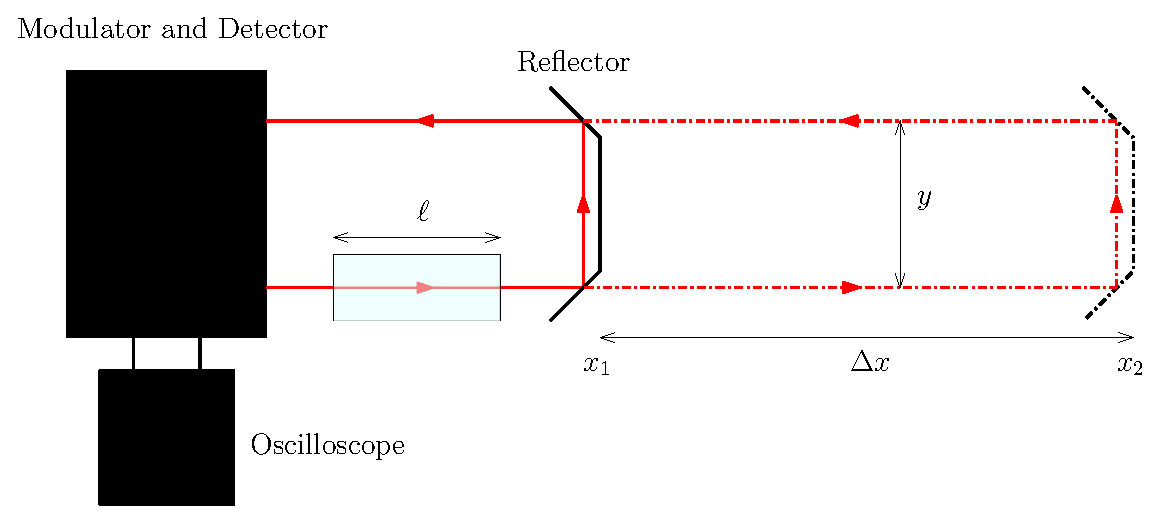
\includegraphics[scale=0.8]{./oscill.eps}
        \end{center}
        \caption{The path followed by the light beam. The second configuration is shown with dashed lines, and should have the blue slab removed.
        The optical path difference between the initial and final configurations is $2\Delta x - (n - 1)\ell$. For the first experiment measuring 
        the speed of light (without the slab, i.e.\ set $\ell = 0$), the path difference is simply $\Delta x$.}
        \label{fig:oscill}
        \end{figure}
        

        Since the frequency of visible light is very high (which means that the wavelength is very low), we modulate its amplitude at a more manageable
        frequency, around $f = 50$ MHz. This means that our old wave $\psi$ is enveloped by a wave of frequency $50$ MHz, so 
        the new wave looks somewhat like
        \[
                \psi_\text{AM} \;=\; A\psi\,\cos{ft}.
        \]
        Thus, the new modulated wave comes in pulses, each of which contains a huge number of oscillations of the original wave.
        Each of these pulses still travels at the speed of light $c$, but the `wavelength' is now $c /f$, which is on the order of a few metres.
        This is on an easily measurable scale.

        This phase difference of $\pi$ corresponds to a path difference of $\lambda /2 = c /2f$. Equating this with the path difference $2\Delta x$,
        we obtain
        \[
                c \;=\; 4f\Delta x.
        \]

        A phase difference between the wave at two different points is observed via an oscilloscope, which plots the signal waveform
        of the waves. A phase difference can be observed simply by looking at both waveforms and seeing how far they are shifted,
        but this is made simpler by using a Lissajous figure.

        \paragraph{Lissajous figures}
        Consider the superposition of the two waves $\sin(\omega t)\,\hat{\textbf{\i}}$ and $\sin(\omega t + \phi)\,\hat{\textbf{j}}$.
        We thus trace a parametric curve in the $xy$ plane, where
        \[
                x = \sin(\omega t), \qquad y = \sin{\omega t}\cos{\phi} + \cos{\omega t}\sin{\phi}.
        \]
        Rearranging and squaring, we obtain
        \[
                (y - x\cos\phi)^2 = \cos^2{\omega t}\sin^2\phi = (1 - x^2)\sin^2\phi.
        \]
        Expanding and rearranging, we finally obtain
        \[
                x^2 + y^2 - 2xy\cos\phi \;=\; \sin^2\phi. 
        \]
        This is the equation of an ellipse, rotated about its center. If the initial waves had different amplitudes, say $A$ and $B$, we simply
        substitute $x \mapsto x /A$ and $y \mapsto y / B$. This preserves the nature of the ellipse. When $\phi = n\pi$, we obtain
        straight lines $x / A = (-1)^n y / B$ (which are just degenerate ellipses).
        Conversely, we can also say that if we change the phase difference $\phi$ such that the Lissajous figure
        has changed from a straight line of positive slope to one of negative slope, we can conclude that $\Delta\phi = \pi$.

        \paragraph{Refractive index calculation}
        Consider a material of refractive index $n$ placed in the path of one of the beams of light such that it crossed a distance of
        $\ell$ through the medium. We adjust the phase difference to a convenient value, say $0$ so that the Lissajous figure is a straight line.
        Let the mirror be at position $x_1$. Now upon removing the medium, the light beam travels a shorter optical path so in order to 
        bring it back to the original phase difference, we move the mirror further away to position $x_2$. Here, we demand that the
        Lissajous figure is exactly the same (straight line with the same slope) as it was previously.

        Now, the removal of the material decreased the path difference by $(n - 1)\ell$, which was exactly compensated by the subsequent
        increase in path difference of $2(x_2 - x_1) = 2\Delta x$. Thus,
        \[
                (n - 1)\ell \;=\; 2\Delta x \,+\, k\lambda.
        \]
        The additional $k\lambda = k c/f$ term arises since our observation is also consistent with an integer multiple of $2\pi$ phase difference,
        i.e.\ an integer multiple of $\lambda = c /f$ path difference. On the other hand, for materials in use such as water and synthetic resin,
        we know that $1 < n < 2$ and $\Delta x < 2$ m, so we deduce that $k = 0$. Thus, we obtain
        \[
                n \;=\; 1 \,+\, \frac{2\Delta x}{\ell}.
        \]
        
        \section{Experimental setup}
        An emitting and receiving unit is setup like in Fig.~\ref{fig:oscill}, with the emitted and received beams focused properly by lenses.
        An angular mirror on an optical bench is used to redirect the light beam. The phase difference between the emitted (modulated at frequency $f$) 
        and received beams is measured by an attached oscilloscope. For the first part, the reflecting mirror is brought close to the mirror and the 
        phase difference is set to zero -- the corresponding Lissajous figure is a straight line with positive slope. The mirror is moved
        further away by $\Delta x$ where the phase difference becomes $\pi$ -- the Lissajous figure is now a straight line with negative slope.
        The speed of light is calculated as $4f\Delta x$.

        For the second part, the refractive material (a tube of water or a synthetic resin slab) is placed in the path of one of the beams
        and the phase difference is set to zero. The material is removed, and the mirror is moved away by $\Delta x$ to restore the phase
        difference of zero. The refractive index of the material is calculated as $1 + 2\Delta x / \ell$, where $\ell$ is the length of the
        material across which the light beam travels.

        The light beam is modulated at a frequency of $f = 50.1$MHz, and the lengths of the water tub and resin slab are $\ell_\text{water} = 100$ cm and 
        $\ell_\text{resin} = 29$ cm respectively.
        
        \section{Experimental data and analysis}
        
        \subsection{Data processing}
        
        All data has been gathered into an Excel spreadsheet, read using \texttt{pandas} and processed using \texttt{numpy}.
        The code used has been listed below.

        \lstinputlisting[language=Python]{calculate.py}

        The means of the displacements $\Delta x = x_2 - x_1$ were calculated for all three sets of data along with their standard errors, listed
        below.
        \begin{center}
        \begin{tabular}{rr}
                $\Delta x_\text{air} =$ & $150.1 \pm 1.0$ cm \\
                $\Delta x_\text{water} =$ & $17.4 \pm 1.2$ cm \\
                $\Delta x_\text{resin} =$ & $7.5 \pm 0.3$ cm \\
        \end{tabular}
        \end{center}

        \subsection{Error Analysis}
        Using standard error propagation formulae, we have
        \[
                \left(\frac{\delta c}{c}\right)^2 = \left( \frac{\delta f}{f} \right)^2 + \left( \frac{\delta(\Delta x)}{\Delta x} \right)^2, \qquad
                \left(\frac{\delta n}{n}\right)^2 = \left( \frac{\delta \ell}{\ell} \right)^2 + \left( \frac{\delta(\Delta x)}{\Delta x} \right)^2, \qquad
                \left(\frac{\delta c_*}{c_*}\right)^2 = \left( \frac{\delta c}{c} \right)^2 + \left( \frac{\delta n}{\Delta n} \right)^2.
        \]

        Since the standard error in measured $\Delta x_\text{resin}$ is very small ($0.3$ cm), this will be outweighed by measurement errors
        on the scale, which we estimate as $0.5$ cm.
        All other errors in measured quantities are taken as the standard errors in the measurements.
        We have also used $\delta f \approx 0.01$ MHz and $\delta\ell \approx 0.5$ cm.

        \subsection{Reported Values}
        We report the following vales, along with standard errors, literature values, errors from the literature value, and percentage errors
        from the literature value for each of the three sets.
        \begin{center}
        \begin{tabular}{lcccc}
        Quantity        & Value with standard error             & Literature value              & Error from literature         & Percentage error
        \\\hline
        $c_\text{air}$  & $(3.008 \pm 0.019) \times 10^8$ m/s   & $2.998 \times 10^8$ m/s       & $+0.010 \times 10^8$ m/s      & $+0.3\%$ \\
        $c_\text{water}$& $(2.233 \pm 0.159) \times 10^8$ m/s   & $2.248 \times 10^8$ m/s       & $-0.015 \times 10^8$ m/s      & $-0.7\%$ \\
        $c_\text{resin}$& $(1.983 \pm 0.137) \times 10^8$ m/s   & $1.877 \times 10^8$ m/s       & $+0.106 \times 10^8$ m/s      & $+5.6\%$ \\
        $n_\text{water}$& $1.347 \pm 0.095$                     & $1.333$                       & $+0.014$                      & $+1.1\%$ \\
        $n_\text{resin}$& $1.517 \pm 0.104$                     & $1.597$                       & $-0.080$                      & $-5.0\%$
        \end{tabular}
        \end{center}
        
        \section{Discussion}
        
        \subsection{Sources of error}
        As suggested, the scale on the optical bench used for measuring $\Delta x$ must be continuous and accurate, which may be verified independently.
        The Lissajous figures must be observed carefully, perhaps by zooming in and increasing the sensitivity.
        The internal circuitry also leads to the appearance of a small interference signal $U_s$, on top of the useful signal $U_n$.
        It is given that the maximum error is approximately $U_s / 2U_n$ -- thus, the larger the useful signal amplitude, the smaller the systematic
        error from this source. Essentially, the diode light should have a good intensity. Again, in the second half of the experiment,
        the refractive material must be placed such that the $y$ signal is of good strength. When a liquid is used, the length $\ell$ must
        exclude the thickness of the container. Our path difference calculation may be refined further if the net thickness $\ell'$ and refractive
        index $n'$ of the container is known -- we then have a path difference $2\Delta x - 2(n - 1)\ell - 2(n' - 1)\ell'$. The last term
        may however be deemed negligeable. Naturally, the container must be perfectly clean and transparent, so if water is used,
        it should be deionized or distilled.

        
        \section{Conclusion}
        In conclusion, we have measured the speed of light in different media by mesuring the distance it covers for a given phase shift.
        This was done with an amplitude modulated wave and the phase difference was observed via an oscilloscope.

        % \nocite{*}
        % \bibliographystyle{plain}
        % \bibliography{ref}

\end{document}
